\documentclass[10pt]{article}
\usepackage[utf8]{inputenc}
\usepackage[spanish]{babel}
\usepackage{graphicx}
\usepackage{listings}
\usepackage{hyperref}
\usepackage{amsmath}
\usepackage{float}
\usepackage{cite}
\usepackage{titling}
\usepackage{graphicx}
\setcounter{secnumdepth}{0}
\usepackage{lineno}
\usepackage{tocloft}  % Paquete para manipular el contenido del índice

% Configuración para mostrar código fuente
\lstset{
    basicstyle=\ttfamily\footnotesize,
    breaklines=true,
    breakatwhitespace=true,
    numbers=left,
    numberstyle=\tiny,
    stepnumber=1,
    numbersep=5pt,
    keywordstyle=\color{blue},
    commentstyle=\color{gray},
    showstringspaces=false
}

\title{Análisis de Métodos de Multiplicación de Matrices}

\author{Gabriel Isaac Valdez Nole\\ \\ Departamento de Matemática \\ y Ciencia de la Computación, \\Universidad de Santiago de Chile, Santiago, Chile}

\date{21 de octubre de 2024}

\begin{document}

\maketitle

\begin{abstract}
En este informe se implementan en lenguaje C diferentes métodos de multiplicación de matrices, variando el orden de los bucles y el acceso a los elementos de las matrices. Se analizan los métodos ijk, jik, ikj, jki, kij, kji, además de estrategias como aplanar la matriz en 1D y usar aritmética de punteros. Se estudia la relación entre el tiempo de ejecución y la manera de acceder a las matrices, y se presentan experimentos que comparan su rendimiento.
\end{abstract}

\section{Introducción}
La multiplicación de matrices es una operación fundamental en matemáticas y computación, con aplicaciones en álgebra lineal, gráficos por computadora, procesamiento de señales y aprendizaje automático, según la referencia \cite{Strang2016}. El tiempo de ejecución de la multiplicación de matrices puede variar dependiendo de cómo se accede a los elementos de las matrices y el orden en que se realizan los bucles anidados según la referencia \cite{Goto2008}.

Este informe analiza diferentes métodos de multiplicación de matrices implementados en lenguaje C, variando el orden de los índices en los bucles (ijk, jik, ikj, jki, kij, kji), además de métodos, como aplanar las matrices en un único puntero, sin tener que usar un doble puntero y el uso de aritmética de punteros. Se analiza cómo estas variaciones varían el tiempo de ejecución debido a las distintas formas de acceso a la matriz.

La estructura del informe es la siguiente, se comienza con una explicación de la multiplicación de matrices. Luego se explica la implementación de los diferentes métodos y se presentan las funciones más relevantes. Seguimos analizando la correctitud de la implementación. Se realiza un análisis de la complejidad temporal y espacial teórica de cada método, finalmente, se presentan los resultados de la variación del tiempo de ejecución de los distintos métodos y conclusiones del análisis de los resultados.

\section{Desarrollo}
En esta sección se describen los fundamentos de la multiplicación de matrices, detalles sobre cómo se manejó la implementación en lenguaje C, correctitud de la implementación, y análisis de la complejidad temporal y espacial de cada uno método.

\subsection{Multiplicación de Matrices}
Dados dos matrices $A \in \mathbb{R}^{M \times K}$ y $B \in \mathbb{R}^{K \times N}$, su producto $C = A \times B$ es una matriz $C \in \mathbb{R}^{M \times N}$ donde cada elemento $c_{ij}$ se calcula como:

\[
c_{ij} = \sum_{k=1}^{N} a_{ik} \cdot b_{kj}
\]

Este cálculo requiere tres bucles anidados, y el orden en que se recorren puede afectar significativamente el rendimiento en cuanto a tiempo de ejecución.

\subsection{Descripción del Código}

El código utilizado en este experimento implementa diferentes métodos de acceder a la matriz para realizar la multiplicación de matrices en lenguaje C.

Primero que todo para los casos donde se accede a la matriz de la forma clásica usando ijk, se almacena la matriz en un doble puntero, asignando memoria con el número de filas y por cada fila se asigna memoria con un largo igual a la cantidad de columnas por cada fila. Esta forma de asignar memoria para la matriz A de orden M*K y la matriz B de orden K*N. Para la matriz resultado la asignación será la misma con el orden M*N. Esta forma de asignar memoria es la misma para el método donde se invierten los ciclos (ijk, jik, ikj, jki, kij, kji).

Esto cambia para el método donde se aplana la matriz y se almacena en un puntero, la asignación de la memoria para las 2 matrices que van a ser multiplicadas ahora pasará a ser del largo del resultado de multiplicar el orden de la matriz, si la matriz A tiene M filas y K columnas, el largo del puntero será la multiplicación de M*K, si la matriz B tiene K filas y N columnas, el largo del puntero será la multiplicación de K*N. Para la matriz resultado, la asignación de memoria será la multiplicación de la cantidad de filas de A y la cantidad de columnas de B, quedando M*N. Para el método donde se aplica la aritmética de punteros la asignación de memoria es la misma porque las matrices se almacenan en un puntero.

A continuación, se describe cada método implementado y la forma en que accede a la matriz.

\begin{enumerate}
    \item \textbf{multiplicar\_i\_j\_k}: En este método se recorre las filas de $A$, luego las columnas de $B$, y finalmente suma sobre $k$. Este es el algoritmo clásico de multiplicación de matrices.
    \item \textbf{multiplicar\_j\_i\_k}: Recorre las columnas de $B$, luego las filas de $A$, y suma sobre $k$.
    \item \textbf{multiplicar\_i\_k\_j}: Recorre las filas de $A$, luego suma sobre $k$, y finalmente recorre las columnas de $B$.
    \item \textbf{multiplicar\_j\_k\_i}: Recorre las columnas de $B$, suma sobre $k$, y luego recorre las filas de $A$.
    \item \textbf{multiplicar\_k\_i\_j}: Suma sobre $k$, luego recorre las filas de $A$, y finalmente las columnas de $B$.
    \item \textbf{multiplicar\_k\_j\_i}: Suma sobre $k$, luego recorre las columnas de $B$, y finalmente las filas de $A$.
    \item \textbf{multiplicar\_1D}: Las matrices se almacenan en arreglos unidimensionales y se accede a los elementos de la matriz mediante fórmulas para acceder a los índices en las matrices aplanadas.
    \item \textbf{multiplicar\_aritmetica\_punteros\_1D}: Se utiliza aritmética de punteros para acceder a los elementos de las matrices aplanadas.
\end{enumerate}

A continuación, se presentarán las funciones más importantes del código utilizado para el experimento. En los siguientes fragmentos de código se basará el cálculo de la complejidad temporal y espacial:

\begin{lstlisting}

void multiplicar_i_j_k(int filas, int fila_columna, int columnas, float **a, float **b, float **c) {

    int i, j, k;

    for (i = 0; i < filas; i = i + 1) {
        for (j = 0; j < columnas; j = j + 1) {
                c[i][j] = 0; 
            for (k = 0; k < fila_columna; k = k + 1) {
                c[i][j] = c[i][j] + a[i][k] * b[k][j];
            }
        }
    }

}

void multiplicar_j_i_k(int filas, int fila_columna, int columnas, float **a, float **b, float **c) {

    int i, j, k;

    for (j = 0; j < columnas; j = j + 1) {
        for (i = 0; i < filas; i = i + 1) {
                c[i][j] = 0; 
            for (k = 0; k < fila_columna; k = k + 1) {
                c[i][j] = c[i][j] + a[i][k] * b[k][j];
            }
        }
    }

}

void multiplicar_i_k_j(int filas, int fila_columna, int columnas, float **a, float **b, float **c) {

    int i, j, k;

    for (i = 0; i < filas; i = i + 1) {
        for (k = 0; k < fila_columna; k = k + 1) {
            for (j = 0; j < columnas; j = j + 1) {
                c[i][j] = c[i][j] + a[i][k] * b[k][j];
            }
        }
    }

}

void multiplicar_j_k_i(int filas, int fila_columna, int columnas, float **a, float **b, float **c) {

    int i, j, k;

    for (j = 0; j < columnas; j = j + 1) {
        for (k = 0; k < fila_columna; k = k + 1) {
            for (i = 0; i < filas; i = i + 1) {
                c[i][j] = c[i][j] + a[i][k] * b[k][j];
            }
        }
    }

}

void multiplicar_k_i_j(int filas, int fila_columna, int columnas, float **a, float **b, float **c) {

    int i, j, k;

    for (k = 0; k < fila_columna; k = k + 1) {
        for (i = 0; i < filas; i = i + 1) {
            for (j = 0; j < columnas; j = j + 1) {
                c[i][j] = c[i][j] + a[i][k] * b[k][j];
            }
        }
    }

}

void multiplicar_k_j_i(int filas, int fila_columna, int columnas, float **a, float **b, float **c) {

    int i, j, k;

    for (k = 0; k < fila_columna; k = k + 1) {
        for (j = 0; j < columnas; j = j + 1) {
            for (i = 0; i < filas; i = i + 1) {
                c[i][j] = c[i][j] + a[i][k] * b[k][j];
            }
        }
    }

}

void multiplicar_1D(int filas, int fila_columna, int columnas, float *a_1D, float *b_1D, float *c_1D) {

    int i, j, k;

    for (i = 0; i < filas; i = i + 1) {
        for (j = 0; j < columnas; j = j + 1) {
                c_1D[i * columnas + j] = 0; 
            for (k = 0; k < fila_columna; k = k + 1) {
                c_1D[i * columnas + j] = c_1D[i * columnas + j] + a_1D[i * fila_columna + k] * b_1D[k * columnas + j];
            }
        }
    }

}

void multiplicar_aritmetica_punteros_1D(int filas, int fila_columna, int columnas, float *a, float *b, float *c) {

    int i, j, k;

    for (i = 0; i < filas; i = i + 1) {
        for (j = 0; j < columnas; j = j + 1) {
                *(c + i * columnas + j) = 0; 
            for (k = 0; k < fila_columna; k = k + 1) {
                *(c + i * columnas + j) = *(c + i * columnas + j) + (*(a + i * fila_columna + k)) * (*(b + k * columnas + j));
            }
        }
    }

}
\end{lstlisting}

\subsection{Correctitud de la Implementación}

Para verificar la correctitud de las implementaciones, se utilizaron matrices cuadradas de tamaño $N \times N$ llenas con el valor $1$. Al multiplicar dos matrices de unos, el resultado es una matriz donde cada elemento es igual a $N$, ya que:

\[
c_{ij} = \sum_{k=1}^{N} 1 \times 1 = N
\]

Se realizaron pruebas con diferentes tamaños de $N$ y se verificó que todas las implementaciones producen el resultado correcto, es decir, una matriz llena de $N$ en todas sus celdas.

\subsection{Análisis de Complejidad Temporal y Espacial}

Se analizará la complejidad temporal con el peor caso, el cual es multiplicar matrices cuadradas porque se tiene que recorrer N filas y N columnas lo que por consecuente aumenta la carga a diferencia de multiplicar matrices no cuadradas, ya que tendría que recorrer menos elementos, por último la complejidad espacial de cada método.

\subsubsection{Método 1: \texttt{multiplicar\_i\_j\_k},\\
Método 2: \texttt{multiplicar\_j\_i\_k},
Método 3: \texttt{multiplicar\_i\_k\_j},\\
Método 4: \texttt{multiplicar\_j\_k\_i},
Método 5: \texttt{multiplicar\_k\_i\_j},\\
Método 6: \texttt{multiplicar\_k\_j\_i}
}

\paragraph{Complejidad Temporal}

La complejidad temporal en el peor caso es $O(N \times N \times N)$, donde $N$, $N$, $N$ son las dimensiones de las matrices. La complejidad es $O(N^3)$, ya que se usan 3 ciclos for anidados para moverse entre las filas y columnas, además del que mantiene los productos parciales.

Esto se fundamenta en el código, al tener tres bucles anidados, donde los límites son los tamaños de las matrices.

\paragraph{Complejidad Espacial}

La complejidad espacial considerando que estamos usando matrices cuadradas de tamaño $N \times N$, y que cada elemento es de tipo \texttt{float} (4 bytes), tenemos:\\

- Matriz $A$: $N \times N \times 4$ bytes\\
- Matriz $B$: $N \times N \times 4$ bytes\\
- Matriz $C$: $N \times N \times 4$ bytes\\
- Variables enteras \texttt{i}, \texttt{j}, \texttt{k}: 3 variables $\times$ 4 bytes = 12 bytes\\
\[
\text{Memoria total} = 3 \times N^2 \times 4 \text{ bytes} + 12 \text{ bytes} = 12N^2 + 12 \text{ bytes}
\]

Por lo tanto, la complejidad espacial es $O(N^2)$.

\subsubsection{Método 7: \texttt{multiplicar\_1D}, Método 8: \texttt{multiplicar\_aritmetica\_punteros\_1D}}

La complejidad temporal sigue siendo $O(N^3)$, porque aunque se almacene de forma distinta la matriz, se siguen utilizando 3 for anidados para mover filas, columna y los productos parciales pero accediendo a la matriz con fórmulas para calcular índices.

\paragraph{Complejidad Espacial}

Las matrices aplanadas ya no ocuparán un doble puntero pero la cantidad de memoria sigue siendo la misma.

- Matriz $A$: $N^2 \times 4$ bytes
- Matriz $B$: $N^2 \times 4$ bytes
- Matriz $C$: $N^2 \times 4$ bytes
- Variables enteras \texttt{i}, \texttt{j}, \texttt{k}: 3 variables $\times$ 4 bytes = 12 bytes

\[
\text{Memoria total} = 3 \times N^2 \times 4 \text{ bytes} + 12 \text{ bytes} = 12N^2 + 12 \text{ bytes}
\]

Por lo tanto, la complejidad espacial es $O(N^2)$.

Resumiendo, todos los métodos tienen una complejidad temporal teórica de $O(N^3)$ y una complejidad espacial de $O(N^2)$. Sin embargo, el rendimiento en cuanto a tiempo de ejecución puede variar debido a la forma en que se accede a la matriz y la eficiencia en el uso de la caché de la memoria, en la siguiente sección se analizará cómo varían los tiempos de ejecución con los distintos métodos que se implementaron, aunque teóricamente.

\subsection{Experimentos y Resultados}

Se realizaron experimentos con el peor caso para medir el tiempo de ejecución de cada método con matrices cuadradas para lograr el número máximo de operaciones en una matriz. Se utilizó la función \texttt{clock()} de la librería \texttt{time.h} para medir el tiempo de CPU en segundos.\\

Los tamaños de las matrices utilizadas se mostrarán algunos datos en el cuadro \ref{tab:datos} con sus tiempos de ejecución usados para crear la figura \ref{fig:tiempo_ejecucion}. Las matrices fueron llenadas con el valor $1$ en todas sus posiciones, ya que independiente del número que se coloca, la cantidad de operaciones sigue siendo la misma y como se mencionó anteriormente colocando puros 1, comprobar que el programa da resultados correctos es intuitivo. Finalmente, se midió el tiempo de ejecución de cada método para realizar el gráfico que se muestra en la figura \ref{fig:tiempo_ejecucion}.

\begin{table}[h!]
\centering
\setlength{\tabcolsep}{4pt} % Ajustar espacio entre columnas
\renewcommand{\arraystretch}{1.2} % Ajustar altura de las filas
\begin{tabular}{|c|c|c|c|c|c|c|c|c|}
\hline
\textbf{Orden} & \textbf{ijk} & \textbf{jik} & \textbf{ikj} & \textbf{jki} & \textbf{kij} & \textbf{kji} & \textbf{1D} & \textbf{aritPunte} \\ \hline
500  & 0.35 & 0.34 & 0.33 & 0.39 & 0.32 & 0.38 & 0.38 & 0.38 \\ \hline
750  & 1.19 & 1.18 & 1.11 & 1.33 & 1.08 & 1.31 & 1.32 & 1.30 \\ \hline
2500 & 63.25 & 55.90 & 41.18 & 117.83 & 40.37 & 97.73 & 61.63 & 61.17 \\ \hline
2750 & 84.53 & 72.02 & 54.51 & 151.96 & 53.81 & 154.33 & 91.42 & 94.97 \\ \hline
3000 & 124.87 & 104.26 & 70.82 & 219.18 & 69.93 & 192.17 & 98.49 & 101.75 \\ \hline
3250 & 161.37 & 137.79 & 90.01 & 257.55 & 88.99 & 282.05 & 168.96 & 167.74 \\ \hline
4500 & 362.38 & 388.83 & 239.00 & 632.75 & 234.28 & 648.50 & 406.73 & 399.95 \\ \hline
4750 & 516.94 & 385.16 & 284.14 & 796.31 & 276.36 & 752.14 & 514.84 & 507.42 \\ \hline
5000 & 589.49 & 556.56 & 330.99 & 1053.32 & 324.48 & 991.09 & 536.66 & 526.06 \\ \hline
\end{tabular}
\caption{Tiempos de ejecución redondeados a dos decimales con sus respectivos órdenes y método usado.}
\label{tab:datos}
\end{table}

\begin{figure}[H]
    \centering
    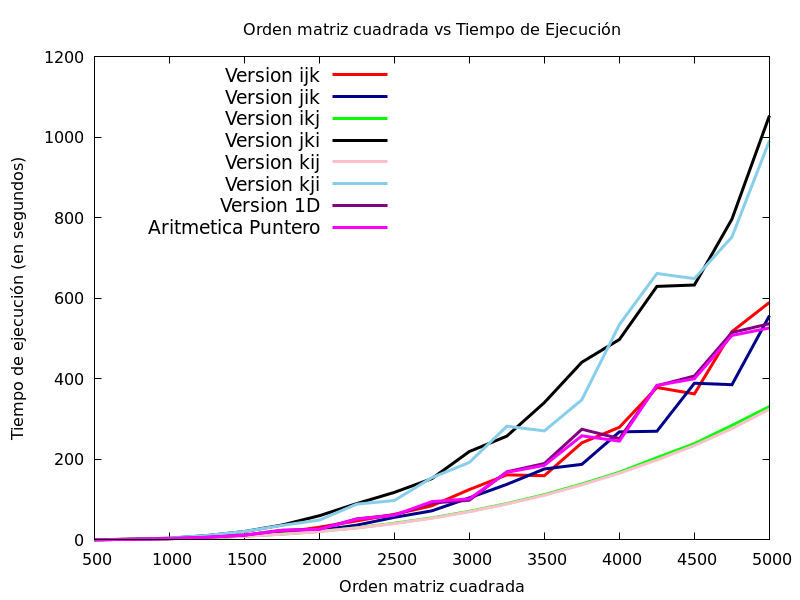
\includegraphics[width=0.8\textwidth]{grafico.png}
    \caption{Tiempo de ejecución vs orden de matriz cuadrada}
    \label{fig:tiempo_ejecucion}
\end{figure}

El tiempo de ejecución más bajo es de los métodos \texttt{\_i\_k\_j} y \texttt{\_k\_i\_j} en comparación con los otros métodos. Se puede explicar cómo estos métodos acceden a la memoria y procesan los datos para justificar los resultados obtenidos. Se detallan los aspectos clave que justifican su eficiencia respecto a los demás métodos.\\

En el método \texttt{i\_k\_j}, se recorre primero la fila \texttt{i}, luego la dimensión intermedia \texttt{k}, y finalmente la columna \texttt{j}. Este orden asegura un acceso secuencial a las filas de \texttt{a} y \texttt{c}, maximizando la eficiencia.\\

En el método \texttt{k\_i\_j}, el índice \texttt{k} fija una fila de \texttt{a} y una columna de \texttt{b}, que son reutilizadas en múltiples iteraciones. Esto optimiza la reutilización de datos ya cargados en la caché.\\

En los demás métodos donde se permutan los índices de la multiplicación clásica, las filas/columnas se acceden de forma discontinua, lo que genera fallos de caché frecuentes.\\

En el caso de la multiplicación accediendo a los datos con fórmulas de índice para aplanar la matriz en 1D, el tiempo de ejecución sube porque tiene que realizar un cálculo extra para calcular el índice en 1D en la matriz original. De forma similar el tiempo de ejecución sube en la aritmética de punteros ya que de igual forma se necesita acceder a las posiciones pero ahora se hace moviéndose a nivel de punteros.\\

\section{Conclusión}

Según las pruebas realizadas, se puede observar cómo varía el tiempo de ejecución aunque los métodos tengan la misma complejidad teórica, ya que 
la manera de acceder a los elementos de las matrices tiene un impacto significativo en el rendimiento de la multiplicación de matrices. Finalmente se puede concluir que los métodos que mejoran la localización de la memoria y reducen las escrituras en memoria pueden aprovechar mejor la jerarquía de caché, resultando en tiempos de ejecución menores.

\section{Bibliografía}

\begin{thebibliography}{9}

\bibitem{Strang2016}
Strang, G. (2016). \textit{Introduction to Linear Algebra}. Wellesley-Cambridge Press. Disponible en: \url{http://math.mit.edu/~gs/linearalgebra/}

\bibitem{Goto2008}
Goto, K., \& van de Geijn, R. A. (2008). Anatomy of High-Performance Matrix Multiplication. \textit{ACM Transactions on Mathematical Software (TOMS)}, 34(3), 1–25. Disponible en: \url{https://www.cs.utexas.edu/~pingali/CS378/2008sp/papers/gotoPaper.pdf?utm_source}

\end{thebibliography}

\end{document}
